\chapter{Lecture 11: The Residue Theorem \& Applications} % Main chapter title

\begin{theorem}
    [Residue Theorem]
    Suppose $f$ is analytic on a simply connected domain $D$, except for a finite number of isolated singularities at $z_1, z_2, \cdots, z_n \in D$. Let $\gamma$ be a piecewise $C^1$, positively oriented, simple closed curve in $D$ which does not pass through any of the singularities. Then:
    \begin{equation}
        \boxed{\oint_{\gamma} f(z) dz = 2\pi i \sum_{z_k \text{ inside } \gamma} \text{Res}(f, z_k)}
    \end{equation}
\end{theorem}
\begin{figure}[H]
    \centering
    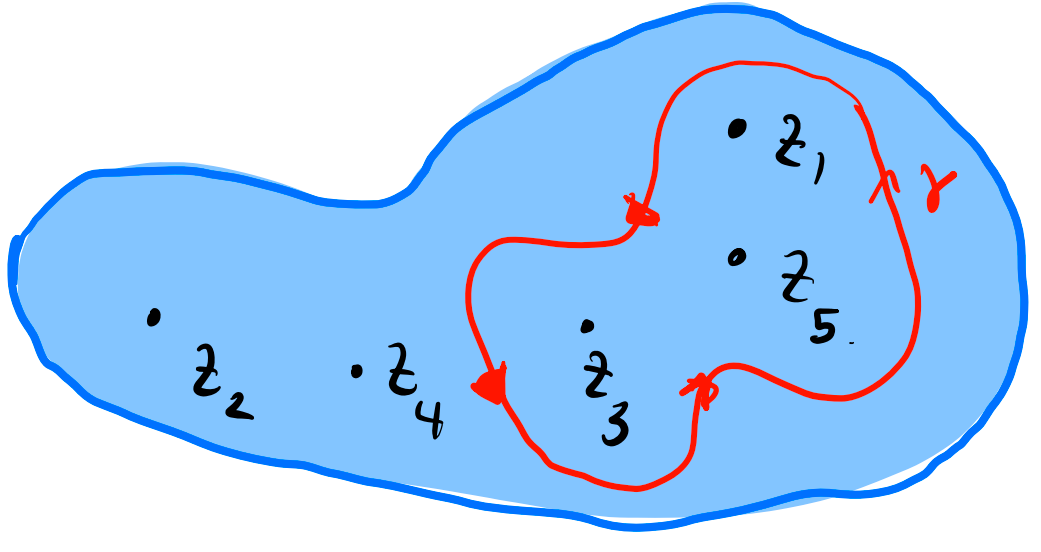
\includegraphics[width=0.4\textwidth]{LECTURE_11/residues.png}
    \caption{Residue Theorem}
    \label{fig:residue}
\end{figure}

\begin{proof}
    We'll use Green's Theorem with $\gamma = \partial \Omega$ where $\Omega$ is the region enclosed by $\gamma$.
    \begin{align*}
        \int_{\partial \Omega} f dz = i \int\int_{\Omega} \left( \frac{\partial f}{\partial x} - i\frac{\partial f}{\partial y} \right) dxdy
    \end{align*}
    We know that the integral of an analytic function over a closed curve is zero, so the only contributions to the integral are from the singularities inside $\Omega$. Let $\gamma_1, \gamma_2, \cdots, \gamma_n$ be disjoint, positively oriented, circles around singularities $z_1, z_2, \cdots, z_n$ respectively. We apply Green's theorem to get:
    \begin{equation*}
        \oint_{\gamma} f(z) dz = \sum_{k : z_k \text{ inside } \gamma} \oint_{\gamma_k} f(z) dz
    \end{equation*}
    \begin{figure}[H]
        \centering
        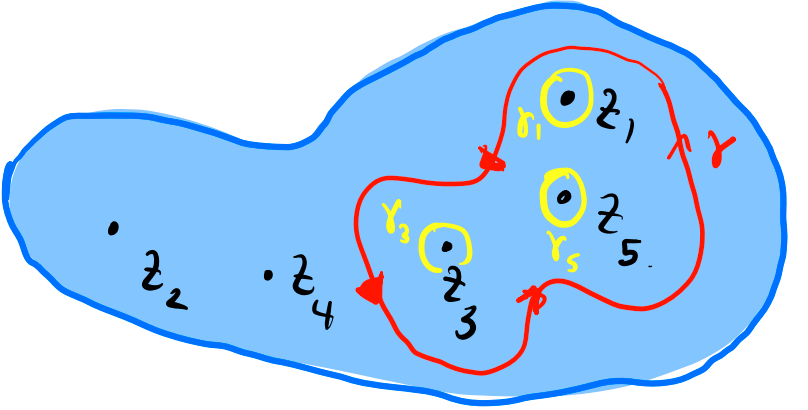
\includegraphics[width=0.4\textwidth]{LECTURE_11/residues-2.png}
        \caption{circles around $z_1, z_2, \cdots, z_n$}
        \label{fig:residue-2}
    \end{figure}

    To compute $\oint_{\gamma_k} f(z) dz$, we can write $f(z)$ as a Laurent series about $z_k$:
    \begin{equation}
        f(z) = \sum_{n = -\infty}^{\infty} a_n (z - z_k)^n = \frac{\text{Res}(f, z_k)}{z - z_k} + \text{regular terms}
    \end{equation}

    Now, we can compute the integral:
    \begin{align*}
        \oint_{\gamma_k} f(z) dz & = \oint_{\gamma_k} \frac{\text{Res}(f, z_k)}{z - z_k} dz + \oint_{\gamma_k} \text{regular terms } dz \\
    \end{align*}
    $\oint_{\gamma_k} \text{regular terms } dz$ is zero because when $n > -1$ the integrand is analytic and thus the integral of an analytic function over a closed curve is zero. When $n < -1$, the integrand is oscillatory and the integral is zero. So we are left with:
    \begin{align*}
        \oint_{\gamma_k} f(z) dz & = \oint_{\gamma_k} \frac{\text{Res}(f, z_k)}{z - z_k} dz \\
    \end{align*}
    Which resembles the Cauchy Integral Formula.
    \begin{align*}
        2\pi i f(z_0) & = \oint_{\gamma} \frac{f(z)}{z - z_0} dz
    \end{align*}
    So we can write:
    \begin{align*}
        \oint_{\gamma_k} f(z) dz & = \oint_{\gamma_k} \frac{\text{Res}(f, z_k)}{z - z_k} dz \\
                                 & = 2\pi i \text{Res}(f, z_k)
    \end{align*}
    Summing over all $z_k$ inside $\gamma$:
    \begin{align*}
        \oint_{\gamma} f(z) dz & = \sum_{k : z_k \text{ inside } \gamma} \oint_{\gamma_k} f(z) dz \\
                               & = 2\pi i \sum_{z_k \text{ inside } \gamma} \text{Res}(f, z_k)
    \end{align*}
\end{proof}

\begin{example}
    Compute:
    \begin{equation*}
        \int_{-\infty}^{\infty} \frac{x^2}{((1 + x^2)(4+ x^2))} dx
    \end{equation*}

    \textbf{Step 1:} Change to a complex integral:
    \begin{equation*}
        P(z) = z^2, \quad Q(z) = (1 + z^2)(4 + z^2)
    \end{equation*}

    \textbf{Step 2:} Choose a contour:
    \begin{figure}[H]
        \centering
        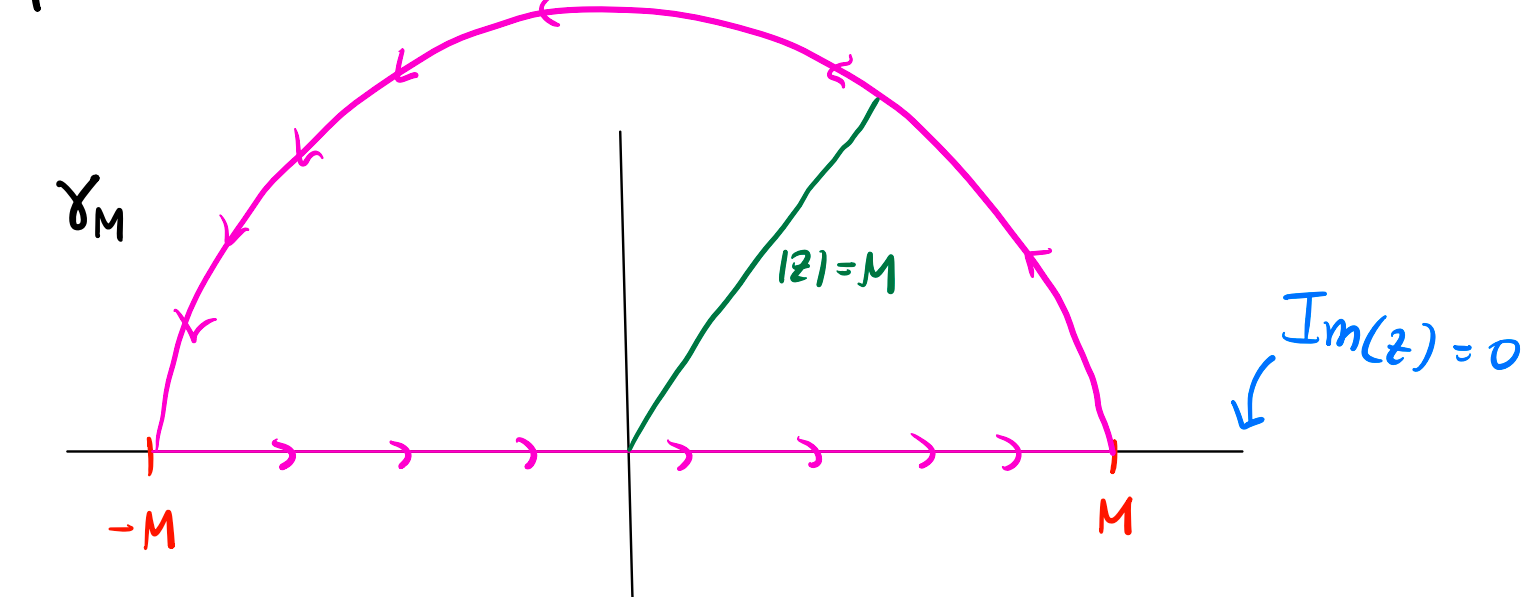
\includegraphics[width=0.4\textwidth]{LECTURE_11/contour.png}
        \caption{Contour}
        \label{fig:contour}
    \end{figure}
    Suppose $M$ is very large
    \begin{enumerate}
        \item $\int_{\gamma_M} \frac{P(z)}{Q(z)} dz$ can be computed by the residue formula.
        \item On the other hand:
              \begin{equation*}
                  \int_{\gamma_M} \frac{P(z)}{Q(z)} dz = \underbrace{\int_{-M}^{M}\frac{x^2}{(1 + x^2)(4 + x^2)} dx}_{\text{The integral we want}} + \int_{0}^{\pi} \frac{P(M e^{i\theta})}{Q(M e^{i\theta})} i M e^{i\theta} d\theta
              \end{equation*}
    \end{enumerate}
    \underline{Now}:
    \begin{align*}
        |P(Me^{i\theta})| & \leq M^2                                                \\
        |Q(Me^{i\theta})| & = |(Me^{i\theta})^2 + 1||(Me^{i\theta})^2 + 4|          \\
                          & \geq \frac{1}{10} M^4 \qquad \text{for a very large } M
    \end{align*}
    \underline{So}
    \begin{equation*}
        \left| \int_0^\pi \frac{P(Me^{i\theta})}{Q(Me^{i\theta})} i M e^{i\theta} d\theta \right| \leq 10 \pi \frac{M^3}{M^4} \to 0 \quad \text{as } M \to \infty
    \end{equation*}
    \textbf{\underline{Thus}}
    \begin{equation*}
        \int_{-\infty}^{\infty} \frac{x^2}{(1 + x^2)(4 + x^2)} dx = \lim_{M \to \infty} \int_{\gamma_M} \frac{P(z)}{Q(z)} dz
    \end{equation*}
    Which can be computed using the residue formula. \\
    $Q(z)$ has zeroes at $z = \pm i, \pm 2i$. only $+i, +2i$ are inside $\gamma_M$ for large $M$. So:
    \begin{align*}
        \boxed{z = i} \quad \rightarrow\quad \frac{z^2}{(z + i)(z-i)(z^2 + 4)}  & = \frac{1}{z - i}\left[\frac{z^2}{(z + i)(z^2 + 4)}\right]   \\
        \text{So Res}(f, i)                                                     & = \frac{i^2}{(i + i)(i^2 + 4)} = \frac{-1}{6i}               \\
        \boxed{z = 2i}\quad \rightarrow \quad \frac{z^2}{(z + i)(z-i)(z^2 + 4)} & = \frac{1}{z - 2i}\left[\frac{z^2}{(z + 2i)(z^2 + 1)}\right] \\
        \text{So Res}(f, 2i)                                                    & = \frac{-4}{4i(-4 + 1)} = \frac{1}{3i}
    \end{align*}
    \underline{Thus, } for a large $M$:
    \begin{align*}
        \int_{\gamma_M} \frac{P(z)}{Q(z)} dz & = 2\pi \left(\frac{-1}{6i} + \frac{1}{3i}\right) \\
                                             & = \frac{\pi}{3}
    \end{align*}
\end{example}

\begin{theorem}
    [Solving Residue Problems]
    \underline{What do we need?} \\
    Polynomials $P(z), Q(z)$ such that:
    \begin{enumerate}
        \item $Q(z)$ has no zeroes on the line $\Re(z) = 0$.
        \item[] Why?
              \begin{itemize}
                  \item To apply the Residue Theorem to the contour shown in figure \ref{fig:contour}.
              \end{itemize}
        \item $\deg(Q) \geq \deg(P) + 2$.
        \item[] Why?
              \begin{itemize}
                  \item To ensure that the integral over the arc goes to zero.
                  \item $\int_0^\pi \frac{P(Me^{i\theta})}{Q(Me^{i\theta})} i M e^{i\theta} d\theta \to 0$ as $M \to \infty$.
              \end{itemize}
    \end{enumerate}

\end{theorem}

\begin{proposition}
    $P, Q$ polynomials that are real-valued on $\Im(z) = 0$ and $\deg(Q) \geq \deg(P) + 2$, then if $Q(x) \neq 0$ for all $x \in \mathbb{R}$, then:
    \begin{equation}
        \int_{-\infty}^{\infty} \frac{P(x)}{Q(x)} dx = 2\pi i \sum_{z_j \in U} \text{Res}\left(\frac{P(z)}{Q(z)}, z_j\right)
    \end{equation}
    Where $ U = \{z_j : \Im(z_j) > 0\}$.
    \label{prop:residue}
\end{proposition}

\begin{proof}
    Take the contour $\gamma_M$ as shown in figure \ref{fig:contour}, for a large $M$, the residue theorem applies and all zeroes of $Q \in \{z : \Im(z) > 0\}$ are inside $\gamma_M$. \\
    \underline{\textbf{Claim:}} for $M$ large:
    \begin{itemize}
        \item $|Q(Me^{i\theta})| \geq c_1M^{\deg(Q)}$ for some $c_1 > 0$.
        \item $|P(Me^{i\theta})| \leq c_2M^{\deg(P)}$ for some $c_2 > 0$.
    \end{itemize}
    This can be proved using the triangle inequality:
    \begin{align*}
        PERFORM THE INEQUALITY
    \end{align*}
    Since $\deg(P) + 1 - \deg(Q) \leq -1$ by assumption. \\
    Now apply the residue theorem to $\gamma_M$:
    \begin{align*}
        \int_{\gamma_M} \frac{P(z)}{Q(z)} dz         & = 2\pi i \sum_{z_j \in U} \text{Res}\left(\frac{P(z)}{Q(z)}, z_j\right) \\
        \int_{-\infty}^{\infty} \frac{P(x)}{Q(x)} dx & = 2\pi i \sum_{z_j \in U} \text{Res}\left(\frac{P(z)}{Q(z)}, z_j\right)
    \end{align*}
\end{proof}

\section{Integrals Involving Trigonometric Functions}

\begin{proposition}
    Suppose $R$ is a rational function (ratio of two polynomials) that is real on $\Im(z) = 0$. We can integrate $(x)\sin(x)$ or $R(x)\cos(x)$ over $(-\infty, \infty)$ by integrating
    $$\Re{R(z)e^{iz}}, \quad \Im{R(z)e^{iz}}$$
    Respectively over the contour shown in figure \ref{fig:contour}.
\end{proposition}

\begin{example}
    Compute:
    $$\int_{-\infty}^{\infty} \frac{\cos(x)}{x^2 + \alpha^2} dx \quad \text{for } \alpha > 0$$

    \textbf{Step 1:} Change to a complex integral and replace $\cos(x)$ with $\Re{e^{iz}}$

    \begin{align*}
        P(z) & = e^{iz}         \\
        Q(z) & = z^2 + \alpha^2
    \end{align*}

    \textbf{Step 2:} $\deg(Q) \geq \deg(P) + 2$.
    \begin{align}
        \lim_{z \to \infty} P(z) & = \lim_{z \to \infty} e^{iz} = 1              \\
        \lim_{z \to \infty} Q(z) & = \lim_{z \to \infty} z^2 + \alpha^2 = \infty
        \therefore \deg(Q)       & \geq \deg(P) + 2
    \end{align}

    \textbf{Step 3:} Choose a contour as shown in figure \ref{fig:contour}. Because we satisfy the conditions of proposition \ref{prop:residue}, we can apply it to compute the integral.

    \begin{align}
        \therefore \int_{-\infty}^{\infty} \frac{\cos(x)}{x^2 + \alpha^2} dx & = \Re{\left(\lim_{M\to \infty}\oint_{\gamma_M} \frac{e^{iz}}{z^2 + \alpha^2} dz\right)}               \\
                                                                             & = \Re{\left(2\pi i \sum_{z_j \in U} \text{Res}\left(\frac{e^{iz}}{z^2 + \alpha^2}, z_j\right)\right)}
    \end{align}

    \textbf{Step 4:} Compute the residues:
    $z^2 + \alpha^2 = 0 \implies z = \pm i\alpha$ and only $i\alpha$ is in $\gamma_M$ for large $M$.
    \begin{align}
        \text{Res}\left(\frac{e^{iz}}{z^2 + \alpha^2}, i\alpha\right) & = \lim_{z \to i\alpha} (z - i\alpha)\frac{e^{iz}}{z^2 + \alpha^2} \\
                                                                      & = \frac{e^{i(i\alpha)}}{2i\alpha} = \frac{e^{-\alpha}}{2i\alpha}
    \end{align}

    \textbf{Step 5:} Compute the integral:

    \begin{align}
        \int_{-\infty}^{\infty} \frac{\cos(x)}{x^2 + \alpha^2} dx & = \Re{\left(2\pi i \sum_{z_j \in U} \text{Res}\left(\frac{e^{iz}}{z^2 + \alpha^2}, z_j\right)\right)} \\
                                                                  & = \Re{\left(2\pi i \frac{e^{-\alpha}}{2i\alpha}\right)}                                               \\
                                                                  & = \frac{\pi e^{-\alpha}}{\alpha}
    \end{align}
\end{example}

\subsection{There is another example in the notes... But I'm tired....}